\documentclass[final,t]{beamer}
\mode<presentation>{\usetheme{PICB}}

% additional settings
\setbeamerfont{itemize}{size=\normalsize}
\setbeamerfont{itemize/enumerate body}{size=\normalsize}
\setbeamerfont{itemize/enumerate subbody}{size=\normalsize}

% additional packages
\usepackage{times}
\usepackage{amsmath,amsthm, amssymb, latexsym}
\usepackage{exscale}
%\boldmath
\usepackage{booktabs, array}
%\usepackage{rotating} %sideways environment
\usepackage[english]{babel}
\usepackage[latin1]{inputenc}
\usepackage[orientation=portrait,size=a1]{beamerposter}
\listfiles
\graphicspath{{figures/}}
% Display a grid to help align images
% \beamertemplategridbackground[1cm]

\title{A Unifying Theory for\\[0.4ex]Experimental Symbolomics}

\author[Sample et al.]{John Sample, Mike Test and Mary Try}

\institute[PICB Shanghai]{Research Group for Experimental Symbolomics\\[0.4ex]
CAS-MPG Partner Institute and Key Laboratory for Computational Biology\\[0.4ex]
Shanghai Institutes for Biological Sciences, Shanghai, China}

\date[Aug. 31 , 2009]{Aug. 31 , 2009}

\newcommand{\footlinetext}{Contact: \{johnsample,miketest,marytry\}@picb.ac.cn \hskip2cm WWW: http://www.picb.ac.cn/Symbolomics}

% abbreviations
\usepackage{xspace}
\makeatletter
\DeclareRobustCommand\onedot{\futurelet\@let@token\@onedot}
\def\@onedot{\ifx\@let@token.\else.\null\fi\xspace}
\def\eg{{e.g}\onedot} \def\Eg{{E.g}\onedot}
\def\ie{{i.e}\onedot} \def\Ie{{I.e}\onedot}
\def\cf{{c.f}\onedot} \def\Cf{{C.f}\onedot}
\def\etc{{etc}\onedot}
\def\vs{{vs}\onedot}
\def\wrt{w.r.t\onedot}
\def\dof{d.o.f\onedot}
\def\etal{{et al}\onedot}
\makeatother

\begin{document}

\begin{frame}{} 

  \begin{columns}[t]    %%%%%%%%%%%%%%%%%%%%%%%%%%%%%%%%%%%%%%

    \begin{column}{.45\linewidth}

      \begin{block}{Overview}
       BUS \( Basic Unsupervised \/ Supervised analysis package \) is a Bioconductor R package able to compute enhanced statistically significant similarities that can be applied to a variety of bioinformatics area  .
      \end{block}

       \begin{block}{Introduction}
        \begin{itemize}
         \item provide computation of both unsupervised and supervised approaches               
         \item computation of similarity using correlation and mutual information \(MI \)
         \item missing-data treatment based on bootstrapping, which allows the treatment of both continuous and discrete data with missing values 
         \item enhanced computation of MI statistical significance, based on fitting the MI distribution on a Beta distribution
         \item efficient correction for multiple hypothesis is achieved through permutations or the MM-correction 
        \end{itemize}
      \end{block}

      \begin{block}{Options Brief Resuming}
            \noindent{\hskip1cm\textbf{Imputation}}
                  \begin{itemize}
                     \item \alert{Goal}->Infer plausible missing value
                     \item \alert{Method}->Bootstrapping: Missing data are filled with randomly resampled value added to uniform distributed random noise
                     \item \alert{Profit}->General purpose technique
                          \begin{itemize}
                             \item Work With Both continuos and discrete data
                             \item Avoid erroneous bias in further analysis
                          \end{itemize}   
                  \end{itemize}

      \
                       
          \noindent{\hskip1cm\textbf{MI Computation}}
                 \begin{itemize}
                    \item \alert{Goal}-> Infer association among variables
                    \item \alert{Method}->"How much information X and Y share?"
                    \item \alert{Profit}-> None-liner association
                 \end{itemize}

     \
              
          \noindent{\hskip1cm\textbf{Single Hypothesis P-value of MI}}
               \begin{itemize}
                   \item \alert{Goal}->Compute statistic significance of MI measures  
                   \item \alert{Method}->Extreme (Close to 0) P-values are obtained from a Beta Distribution. Shape Parameters and estimations using 400 randomly generated MI scores and the methods of moments                           
                   \item \alert{Profit}-> Reduced number of permutation compared to other state of art algorithm.                        
               \end{itemize}
               
          \noindent{\hskip1cm\textbf{Multiple Hypothesis P-value}}
               \begin{itemize}
                   \item \alert{Goal}->Find corrected P-value  
                   \item \alert{Method}->MM-correction approach based on inverse $\chi^{2}$ method does not require permutation, evaluate Beta P-value(s) for every test                          
                   \item \alert{Profit}-> Hight Computational efficiency                       
               \end{itemize}                 
     \end{block}
      
     \begin{block}{Input and Output}
         \begin{itemize}
              \item The algorithm is implemented as an R package BUS freely. It can be used with the arguments for:   
                   \begin{itemize}
                          \item The type of the analysis(supervised/unsupervised)
                          \item The distance metric(correlation/MI)
                          \item The statistical significance selection method(MM-correction/permutations)
                  \end{itemize}
             \item \alert{Input}->Table which rows represent molecules and which columns represent different experiments.
             \item \alert{Output}->Table with genes as rows,and genes or traits as columns, and the cells' content represent the gene-gene or gene-trait association.
        \end{itemize}
     \end{block}
    \end{column}   %%%%%%%%%%%%%%%%%%%%%%%%%%%%%%%%%%%%%%

    \begin{column}{.45\linewidth}

      \begin{block}{Visualisation}
            \vskip1ex
            \centering    
            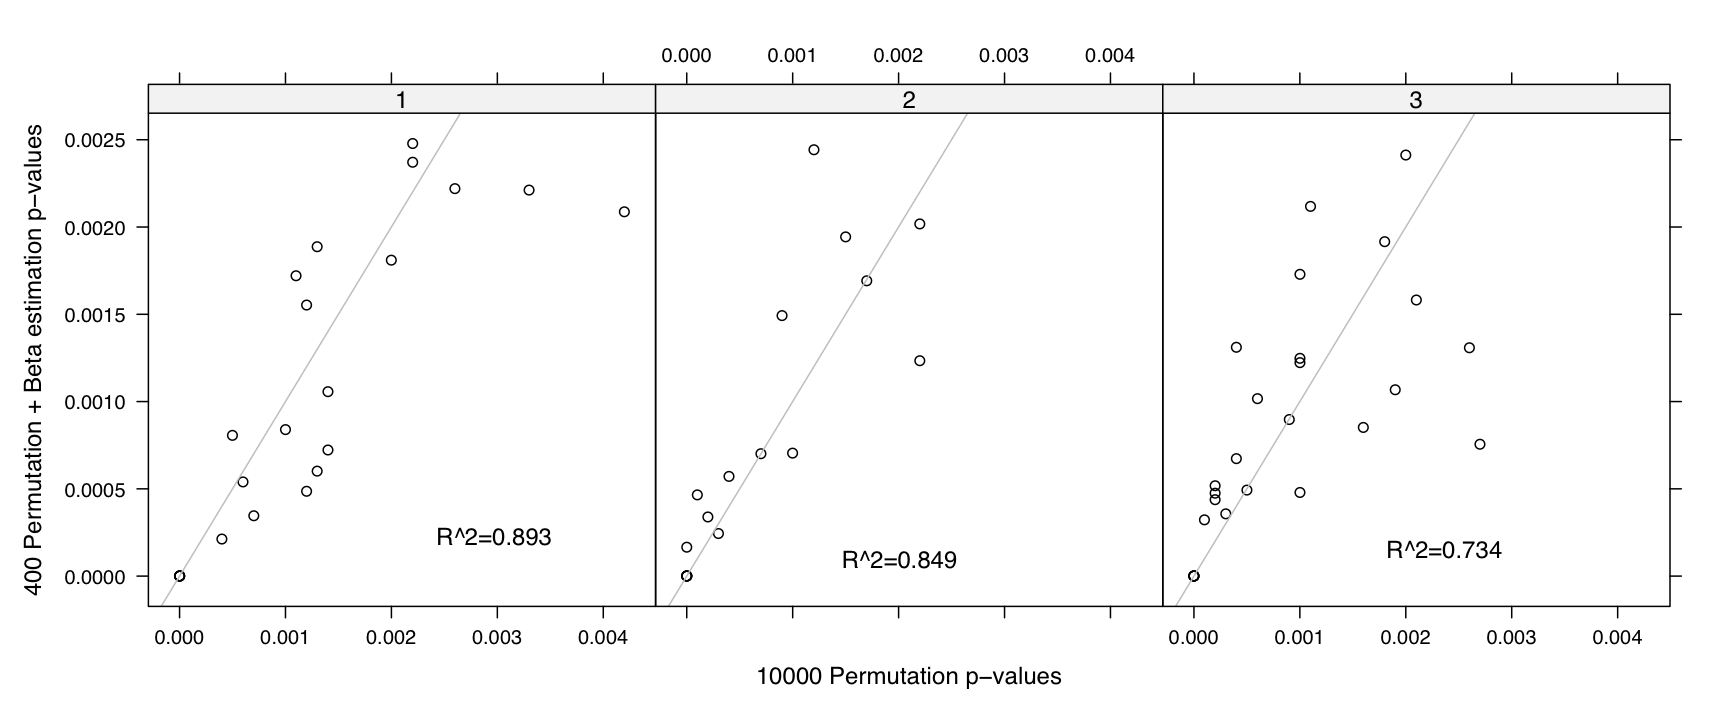
\includegraphics[width=0.9\textwidth]{figure1.png}
            \vskip1ex
              Comparison of p-values obtained using 10000 permutations without Beta Estimation Function and 400 permutations with Beta Estimation Function under di?erent noise levels. The reference gray line has intercept 0 and slope 1. The R2 decreases as the noise level increases}
\label{fig:Beta Estimation Function
      \end{block}


      \begin{block}{Results}
        \vfill
        \noindent{\textbf{Missing Data Filling}}
           \begin{itemize}
               \item The dataset consists of 1705 clones of 22 cancers gene expression data.
                \item We performed simulations that compare the results obtained on complete data (data with no missing values) versus the same data with missing values and then pre-processed with the proposed filling technique, and compared to knn.
                \item In Table linear regression without intercept term is performed to examine the goodness of fit, both methods five good performances across all missing options and metrics used.
            \end{itemize}

        \begin{table}
           \caption{Linear regression without intercept term is performed to examine the goodness of fit, to compare correlation and MI values calculated on data preprocessed using our impute method or knn on data with 5\% genes missing and 25\% traits missing, both versus data with no missing values}
           \begin{tabular}{|c|c|c|c|c|c|c|}
          \hline
         Data&\multicolumn{2}{|c|}{Missing Traits(25 \%)}&\multicolumn{2}{|c|}{Missing Genes(5\%)}&\multicolumn{2}{|c|}{Missing Traints(25\%) and Genes(5\%)}\\
         \hline
         Impute Method&Correlation&MI&Correlation&MI&Correlation&MI\\
         \hline
        Bootstrap&0.983&1&1&0.999&0.981&0.999\\
        \hline
        knn&0.980&1&1&0.999&0.979&0.999\\
       \hline
      \end{tabular}
   \end{table}

        
        \noindent{\textbf{MI p-value}}
            To examine the usefulness of Beta Estimation Function, we compared single p-values 
obtained from a null distribution designed thanks to a limited number of permutations (� 500) for the 
estimation of the parameters and the Beta Estimation Equation for the computation of the p-value, versus 
p-values obtained using 10, 000 permutations.

\

To identify the minimum number of permutation needed to reliably predict the MI distribution, we:
        \begin{itemize}
        \item In each simulation we generated and sorted n + 1 (n number of permutations) independent random numbers with B($\alpha$,$\beta$) distribution. 
        \item The smaller n numbers were used to estimate the shape parameters ($\alpha$,$\beta$) and the right-hand side p-value of the largest number was estimated using our Beta Estimation Function. 
        \item The estimated p-value are then compared with their corresponding real cumulative distribution probability with B($\alpha$,$\beta$) distribution.
        \end{itemize}
      \end{block}


    \end{column}

  \end{columns}   %%%%%%%%%%%%%%%%%%%%%%%%%%%%%%%%%%%%%%

\end{frame}

\end{document}


%%% Local Variables: 
%%% mode: latex
%%% TeX-PDF-mode: t
%%% End: 
